\chapter{Лабораторная работа №3. Реализация конечного автомата для управления ЖКИ}

\section{Протокол работы с ЖКИ S162D}

Индикатор ЖКИ S162D (рис. ~\ref{LCD1602}) позволяет одновременно отображать две строки по 16 символов, при этом каждый символ отображается с помощью матрицы точек 5х8. 

\begin{figure}[!ht]
	\centering
	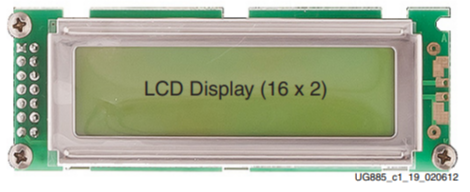
\includegraphics[width=0.4\textwidth]{image/LCD1602.PNG}
	\caption{Внешний вид индикатора S162D}
	\label{LCD1602}
\end{figure}

\begin{table}[!ht]
	\begin{center}
		\begin{tabular}{c c}
			\hline\hline
			Вывод & Назначение \\
			\hline
			VDD & Вывод питания \\
			VSS & Вывод земли \\
			VO & Установка контраста \\
			RS & Сигнал выбора регистра \\
			R/W & Лог. 1 – чтение модуля,лог. 0 – запись в модуль \\
			E & Сигнал выбора модуля \\
			DB0 & Линия информационной шины \\
			DB1 & Линия информационной шины \\
			DB2 & Линия информационной шины \\
			DB3 & Линия информационной шины \\
			DB4 & Линия информационной шины \\
			DB5 & Линия информационной шины \\
			DB6 & Линия информационной шины \\
			DB7 & Линия информационной шины \\
			\hline
		\end{tabular}
		\caption{Выводы индикатора}
		\label{LCD_PIN}
	\end{center}
\end{table}

Выводы VDD и VSS необходимы для подачи питания на индикатор, 
вывод VO служит для настройки контрастности индикатора. Обычно к 
нему подключается скользящий контакт потенциометра на 10-20 
кОм, включенного между линиями питания и земли. Однако при 
известных номиналах можно заменить его обычным резисторным 
делителем

Передача информации на контроллер ЖКИ осуществляется по 
параллельной шине данных DB0…DB7. 
По ней передаются как команды контроллеру, так и коды выводимых символов. 
Вид передаваемой информации (команды или данные) задается 
с помощью вывода 4 (RS): при низком уровне на данном выводе 
контроллер воспринимает принятую информацию как команду, при высоком – как данные. 
Для синхронизации передачи служит вывод 6 (Е) – 
информация с шины данных записывается во входной регистр контроллера 
по спаду сигнала на данном выводе.

Контроллер ЖКИ не только принимает информацию, но и может 
ее передавать – режим чтение/запись устанавливается с помощью 
вывода 5 (R/W): при низком уровне на данном выводе происходит 
запись в контроллер, при высоком – чтение.

\begin{table}[!ht]
	\begin{center}
		\begin{tabular}{c c c c c}
			\hline\hline
			FPGA (U1) Pin & Net Name &  I/O Standard & LCD Header Pin(J31) \\
			\hline
			AT42 & \verb|LCD_DB4_LS| & LVCMOS18 & 4 \\
			AR38 & \verb|LCD_DB5_LS| & LVCMOS18 & 3 \\
			AR39 & \verb|LCD_DB6_LS| & LVCMOS18 & 2 \\
			AN40 & \verb|LCD_DB7_LS| & LVCMOS18 & 1 \\
			AR42 & \verb|LCD_RW_LS| & LVCMOS18 & 10 \\
			AN41 & \verb|LCD_RS_LS| & LVCMOS18 & 11 \\
			AT40 & \verb|LCD_E_LS| & LVCMOS18 & 9 \\
			\hline
		\end{tabular}
		\caption{Подключение индикатора к ПЛИС}
		\label{LCD_TO_FPGA}
	\end{center}
\end{table}

Таким образом, для подключения индикатора к управляющему 
контроллеру необходимо использовать 11 выводов. Для уменьшения 
данного количества возможна работа ЖКИ с 4-проводной шиной 
данных – к ЖКИ подключаются только выводы DB7…DB4, при 
этом передача байта на ЖКИ происходит в два этапа: сначала передаются биты DB7…DB4, затем DB3…DB0. Количество используемых выводов контроллера уменьшается до 7.

Последовательности действий, которые необходимо выполнить 
управляющей системе при совершении операций записи и чтения 
для 4-разрядной шин приведены ниже.

\begin{figure}[!ht]
	\centering
	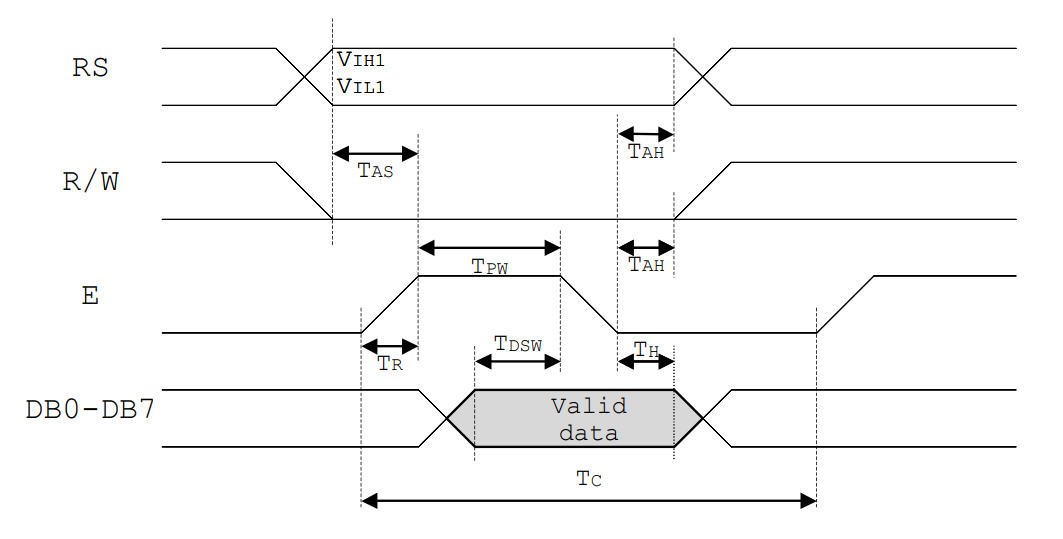
\includegraphics[width=0.7\textwidth]{image/LCD_WR_2.PNG}
	\caption{Временная диаграмма операции записи}
	\label{full_adder}
\end{figure}

\begin{table}[!ht]
	\begin{center}
		\begin{tabular}{c c c c c}
			\hline\hline
			Параметр 							& Обозн. 	& Мин. 	& Макс. \\
			\hline
			Enable Cycle Time, Pin E 			& tC		& 400 	& 	- 	\\
			Enable Pulse Width Pin E 			& tPW 		& 150 	& 	- 	\\
			Enable Rise/Fall Time Pin E 		& tR/tF 	& - 	& 	25	\\
			Address Setup Time Pins: RS,RW,E 	& tAS 		& 30 	& 	-	\\
			Address Hold Time Pins: RS,RW,E 	& tAH 		& 10 	& 	-	\\
			Data Setup Time Pins: DB0 - DB7 	& tDSW 		& 40 	& 	-	\\
			Data Hold Time Pins: DB0 - DB7  	& tH 		& 10 	& 	-	\\
			\hline
		\end{tabular}
		\caption{Временные характеристики сигналов при записи (нс)}
		\label{LCD_TO_FPGA_WR_TABLE}
	\end{center}
\end{table}

Операции записи для 4-разрядной шины:
\begin{enumerate}
	\item Установить значение линии RS.
	\item Вывести значение старшей тетрады байта данных на линии шины DB4...DB7.
	\item Установить линию Е = 1.
	\item Установить линию Е = 0.
	\item Вывести значение младшей тетрады байта данных на линии шины DB4...DB7.
	\item Установить линию Е = 1.
	\item Установить линию Е = 0.
	\item Установить линии шины DB0...DB7 = HiZ.
\end{enumerate}

\begin{figure}[!ht]
	\centering
	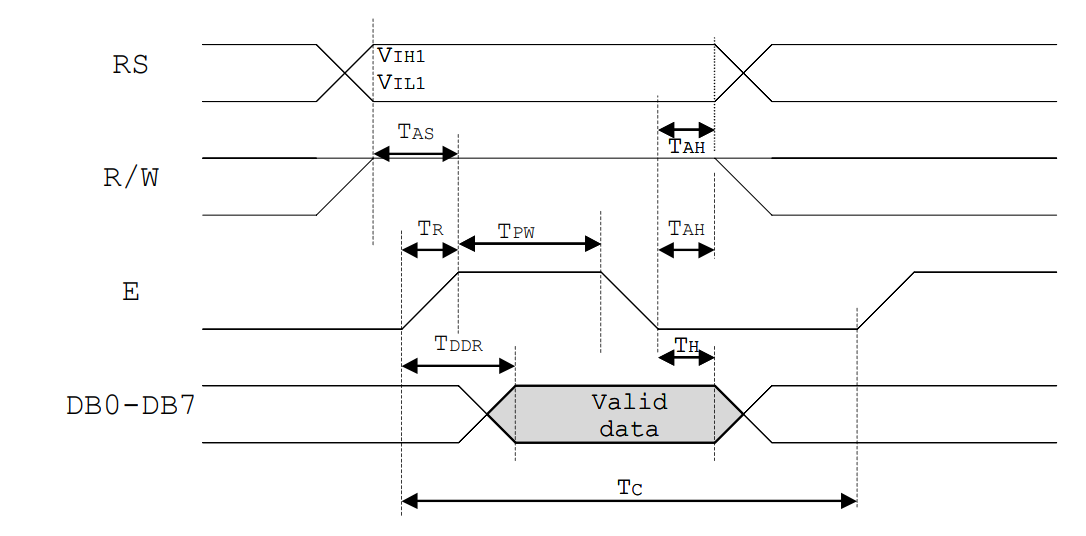
\includegraphics[width=0.7\textwidth]{image/LCD_READ_2.PNG}
	\caption{Временная диаграмма операции чтения}
	\label{full_adder}
\end{figure}

\begin{table}[!ht]
	\begin{center}
		\begin{tabular}{c c c c c}
			\hline\hline
			Параметр 							& Обозн. 	& Мин. 	& Макс. \\
			\hline
			Enable Cycle Time, Pin E 			& tC		& 400 	& 	- 	\\
			Enable Pulse Width Pin E 			& tPW 		& 150 	& 	- 	\\
			Enable Rise/Fall Time Pin E 		& tR/tF 	& - 	& 	25	\\
			Address Setup Time Pins: RS,RW,E 	& tAS 		& 30 	& 	-	\\
			Address Hold Time Pins: RS,RW,E 	& tAH 		& 10 	& 	-	\\
			Data Setup Time Pins: DB0 - DB7 	& tDSW 		&  - 	& 	100	\\
			Data Hold Time Pins: DB0 - DB7  	& tH 		& 10 	& 	-	\\
			\hline
		\end{tabular}
		\caption{Временные характеристики сигналов при чтении(нс)}
		\label{LCD_TO_FPGA_RD_TABLE}
	\end{center}
\end{table}

Операции чтения для 4-разрядной шины:
\begin{enumerate}
	\item Установить значение линии RS.
	\item Установить линию R/W = 1.
	\item Установить линию Е = 1.
	\item Считать значение старшей тетрады байта данных с линий шины DB4...DB7.
	\item Установить линию Е = 0.
	\item Установить линию Е = 1.
	\item Считать значение младшей тетрады байта данных с линий шины DB4...DB7.
	\item Установить линию Е = 0.
	\item Установить линию R/W = 0.
\end{enumerate}

Приведенные операции подразумевают, что время выполнения 
каждого шага составляет не менее 250 нс. 

Описанные операции записи/чтения байта являются базовыми 
для осуществления обмена данными с ЖКИ модулем.

В техническом описании на контроллер ЖКИ приведены алгоритмы инициализации индикатора для различных вариантов его 
подключения. Рассмотрим алгоритм инициализации для подключения по 4-проводной шине данных. Он состоит из следующих этапов:
\begin{enumerate}
	\item При включении ожидание не менее 40 мс после того момента, как напряжение питания превысит 2,7 В.
	\item Отправка команды 0x30.
	\item Ожидание не менее 4,1 мс.
	\item Отправка команды 0х30.
	\item Ожидание не менее 100 мкс.
	\item Отправка команды 0х30. После данной команды контроллер 
выходит на нормальный режим работы: может выполнять данные 
ему инструкции и сигнализировать об их выполнении флагом BF.
	\item  При включении ЖКИ по умолчанию настроен на работу с 8-
разрядной шиной данных, поэтому в первую очередь необходимо 
установить 4-разрядный режим путем установки флага D/L в ноль 
командой 0х20. После данной команды все передачи по шине данных будут проходить в 2 этапа: сначала передача старшей тетрады, 
затем – младшей.
	\item Отправка команды 0х28 – данная команда установит значения флагов N и F таким образом, что ЖКИ будет настроен на отображение двух строк с матрицами символов 5х8 точек
	\item Отправка команды 0х0С – установка значений флагов D, C, 
B – включение отображения на дисплей, символы курсоров не отображаются.
	\item  Отправка команды 0х06 – установка значений флагов I/D и S
– настройка счетчика адреса АС на увеличение при записи символа, 
выключение сдвига экрана при записи.
\end{enumerate}

После выполнения данной последовательности работа с дисплеем заключается в записи по определенным адресам кодов символов, которые необходимо вывести на экран. При приведенных выше настройках при отправке в ЖКИ кода символа он отображается в 
том месте экрана, на которое указывает счетчик АС, – после инициализации он указывает на первый символ первой строки. После записи символа значение счетчика автоматически увеличивается, и он начинает указывать на второй символ. При записи последнего символа первой строки АС автоматически начинает указывать на первый символ второй.

Для непосредственного указания, какой символ требуется переписать, управляющий контроллер отправляет команду, содержащую 
новый адрес АС. Так, адрес первого символа первой строки – 0х00, 
второго – 0х01 и т. д. Однако адреса второй строки, вне зависимости 
от количества знакомест в строке ЖКИ, начинаются с адреса 0х40. 
Далее – 0х41, 0х42 и так по порядку

\section{Разработка конечного автомата для управления ЖКИ}

Изучив основные команды управления ЖКИ и алгоритм его инициализации приступим к разработке модуля упрвления индикатором на языке Verilog. 
Создадим модуль верхнего уровня, который будет генерировать тактовый сигнал требуемой частоты, а также формировать сброс для модуля управления ЖКИ. Используемый тактовый сигнал имеет частоту 200 МГц, 
модуль управления ЖКИ будем тактировать частотой в 50 МГц. Для снижения частоты 
используем примитив \verb|MMCME2_BASE|. Сброс модуля управления ЖКИ будем проводить отслеживая сигнал \verb|LOCKED| примитива \verb|MMCME2_BASE|. 

Входными сигналами модуля будут:
\begin{enumerate}
	\item тактовый сигнал, частотой 200 МГц, который поступает на ПЛИС по дифференциальной паре: \verb|clk_in_n|,\verb|clk_in_p|;
	\item cигнал асинхронного сброса: \verb|rst|.
\end{enumerate}

Выходными сигналами модуля будут: 
\begin{enumerate}
	\item шина данных - \verb|lcd_data|, состоящая из 4 проводов: DB4, DB5, DB6, DB7;  
	\item сигналы управления ЖКИ: \verb|lcd_e|, \verb|lcd_rs|, \verb|lcd_rw|;
	\item сигнал \verb|led| для управления одним светодиодом, предназначен для индикации пристутсвия сигнала сброса и тактового сигнала.
\end{enumerate}

\begin{Verbatim}[tabsize=4]
`timescale 1ns/1ps

module top_lcd(
	// reset
    input wire rst,
    // input clk
    input wire clk_in_p,           
    input wire clk_in_n,
    // leds
	output wire led,
	// LCD data bus
	output wire [3:0] lcd_data, 
	// LCD: E   (control bit)	
	output wire lcd_e,	
	// LCD: RS  (setup or data)
	output wire lcd_rs,	
	// LCD: R/W (read or write)
	output wire lcd_rw	
);

endmodule : top_lcd
\end{Verbatim}

\begin{Verbatim}[tabsize=4]
lcd #(
	.CYCLES_PER_US(50)
)
lcd_inst
(
	.clk(clk_int),  
	.rst(rst_int),  
	.ctrl_lcd({lcd_rs,lcd_rw,lcd_e}),
	.data_lcd(lcd_data)
);
\end{Verbatim}

Создадим модуль, который будет управлять ЖКИ. Входными сигналами модуля будут: тактовый сигнал, сигнал сброса.
Выходными сигналами модуля будут: 
\begin{enumerate}
	\item Шина данных, состоящая из 4 проводов: DB4, DB5, DB6, DB7.  
	\item Шина управления ЖКИ, состоящая из трёх проводов: RS, RW, E.
\end{enumerate}

Также введём параметризацию модуля с помощью параметра \verb|CYCLES_PER_US|, который 
означает число периодов тактового сигнала необходимых для получения задержки
в одну микросекунду. 

\begin{Verbatim}[tabsize=4]

`timescale 1ns/1ps

module lcd #(
	parameter CYCLES_PER_US = 50
)
(
	input wire clk,    
	input wire rst, 
	output wire [2:0] ctrl_lcd,
	output wire [3:0] data_lcd
);
\end{Verbatim}

\begin{Verbatim}[tabsize=4]
	localparam [3:0]
		WAITING = 4'd0,
        INIT_H30_ONE = 4'd1,
        INIT_H30_TWO = 4'd2,
        INIT_H30_THREE = 4'd3,
        INIT_H20 = 4'd4,
        INIT_FUNCTION_SET = 4'd5,
        INIT_DISPLAY_ON = 4'd6,
		INIT_DISPLAY_CLEAR = 4'd7,
		INIT_SET_ENTRY_MODE = 4'd8,
		CUR_FIRST_ROW = 4'd9,
		WRITE_UPPER_LINE = 4'd10,
		COUNTER_UPPER_LINE = 4'd11,
		CUR_SECOND_ROW = 4'd12,
		WRITE_LOWER_LINE = 4'd13,
		COUNTER_LOWER_LINE = 4'd14,
		DONE = 4'd15;
\end{Verbatim}

\begin{Verbatim}[tabsize=4]
	reg [3:0] lcd_state_r;		
	reg [2:0] ctrl_lcd_r; 
	reg [3:0] data_lcd_r;
	
	reg [31:0] counter_r;
	reg [3:0] counter_upper_line_r;
	reg [3:0] counter_lower_line_r;

	reg [7:0] upper_line [15:0];
	reg [7:0] lower_line [15:0];
\end{Verbatim}

\begin{Verbatim}[tabsize=4]
	parameter integer wait__1us = 1 * CYCLES_PER_US;
	parameter integer wait__2us = 2 * CYCLES_PER_US;    // 10us 
	parameter integer wait__3us = 3 * CYCLES_PER_US;    // 20us 
	parameter integer wait__4us = 4 * CYCLES_PER_US;    // 40us 
	parameter integer wait__200us = 200 * CYCLES_PER_US; // 5ms

	parameter integer wait__dispay_clear = 3000 * CYCLES_PER_US; // 1.52ms 
	parameter integer wait__power_on = 15000 * CYCLES_PER_US; // 45ms 

	parameter integer wait__init_h30_one = 5000 * CYCLES_PER_US; // 5ms 
	parameter integer wait__init_h30_two = 500 * CYCLES_PER_US; // 5ms
\end{Verbatim}

\begin{Verbatim}[tabsize=4]
	assign ctrl_lcd = ctrl_lcd_r; // {RS, RW, E} 2, 1, 0
	assign data_lcd = data_lcd_r;
\end{Verbatim}

\begin{Verbatim}[tabsize=4]
	initial begin
		upper_line[0] = 8'h46; // F
		upper_line[1] = 8'h69; // i
		upper_line[2] = 8'h72; // r
		upper_line[3] = 8'h6d; // m
		upper_line[4] = 8'h77; // w
		upper_line[5] = 8'h61; // a
		upper_line[6] = 8'h72; // r
		upper_line[7] = 8'h65; // e
		upper_line[8] = 8'h20; // 
		upper_line[9] = 8'h6c; // l
		upper_line[10] = 8'h6f; // o
		upper_line[11] = 8'h61; // a
		upper_line[12] = 8'h64; // d
		upper_line[13] = 8'h65; // e
		upper_line[14] = 8'h64; // d
		upper_line[15] = 8'h21; // !
				
		lower_line[0] = 8'h30; // 0
		lower_line[1] = 8'h31; // 1
		lower_line[2] = 8'h32; // 2
		lower_line[3] = 8'h33; // 3
		lower_line[4] = 8'h34; // 4
		lower_line[5] = 8'h35; // 5
		lower_line[6] = 8'h36; // 6
		lower_line[7] = 8'h37; // 7
		lower_line[8] = 8'h38; // 8
		lower_line[9] = 8'h39; // 9
		lower_line[10] = 8'h61; // a
		lower_line[11] = 8'h62; // b
		lower_line[12] = 8'h63; // c
		lower_line[13] = 8'h64; // d
		lower_line[14] = 8'h65; // e
		lower_line[15] = 8'h66; // f
	end
\end{Verbatim}

\begin{Verbatim}[tabsize=4]
    always @(posedge clk) begin
        if (rst) begin
        	lcd_state_r <= WAITING;
        	ctrl_lcd_r <= 3'b0;
        	data_lcd_r <= 4'b0;
        	counter_r <= 32'b0;
        	counter_upper_line_r <= 4'b0;
			counter_lower_line_r <= 4'b0;
        end else begin
        	case (lcd_state_r)
        	// Здесь будем описывать конечный автомат
        	endcase
        end
    end
\end{Verbatim}

\begin{Verbatim}[tabsize=4]
WAITING: begin 
	if(counter_r >= wait__power_on) begin
       	lcd_state_r <= INIT_H30_ONE;
          	counter_r <= 32'b0;
    end else begin
   		counter_r <= counter_r + 1;
      	lcd_state_r <= WAITING;
   	end
end
\end{Verbatim}

\begin{Verbatim}[tabsize=4]
INIT_H30_ONE: begin // 0x30
	data_lcd_r <= 4'b0011;
	if(counter_r >= wait__init_h30_one) begin
		counter_r <= 32'b0;
		lcd_state_r <= INIT_H30_TWO;
	end else if(counter_r < wait__init_h30_one && counter_r >= wait__1us) begin
		counter_r <= counter_r + 1;
		ctrl_lcd_r <= 3'b000;
		lcd_state_r <= INIT_H30_ONE;
	end else begin
		counter_r <= counter_r + 1;
		ctrl_lcd_r <= 3'b001;
		lcd_state_r <= INIT_H30_ONE;
	end
end
\end{Verbatim}

\begin{Verbatim}[tabsize=4]
INIT_H30_TWO: begin // 0x30
   	data_lcd_r <= 4'b0011;
   	if(counter_r >= wait__init_h30_two) begin
   		counter_r <= 32'b0;
   		lcd_state_r <= INIT_H30_THREE;
   	end else if(counter_r < wait__init_h30_two && counter_r >= wait__1us) begin
   		counter_r <= counter_r + 1;
   		ctrl_lcd_r <= 3'b000;
   		lcd_state_r <= INIT_H30_TWO;
   	end else begin
   		counter_r <= counter_r + 1;
   		ctrl_lcd_r <= 3'b001;
   		lcd_state_r <= INIT_H30_TWO;
   	end
end
\end{Verbatim}

\begin{Verbatim}[tabsize=4]
INIT_H30_TWO: begin // 0x30
   	data_lcd_r <= 4'b0011;
   	if(counter_r >= wait__init_h30_two) begin
   		counter_r <= 32'b0;
   		lcd_state_r <= INIT_H30_THREE;
   	end else if(counter_r < wait__init_h30_two && counter_r >= wait__1us) begin
   		counter_r <= counter_r + 1;
   		ctrl_lcd_r <= 3'b000;
   		lcd_state_r <= INIT_H30_TWO;
   	end else begin
   		counter_r <= counter_r + 1;
   		ctrl_lcd_r <= 3'b001;
   		lcd_state_r <= INIT_H30_TWO;
   	end
end
\end{Verbatim}

\begin{Verbatim}[tabsize=4]
INIT_H30_THREE: begin // 0x30
	data_lcd_r <= 4'b0011;
	if(counter_r >= wait__200us) begin
		counter_r <= 32'b0;
		lcd_state_r <= INIT_H20;
	end else if(counter_r < wait__200us && counter_r >= wait__1us) begin
		counter_r <= counter_r + 1;
		ctrl_lcd_r <= 3'b000;
		lcd_state_r <= INIT_H30_THREE;
	end else begin
		counter_r <= counter_r + 1;
		ctrl_lcd_r <= 3'b001;
		lcd_state_r <= INIT_H30_THREE;
	end
end
\end{Verbatim}

\begin{Verbatim}[tabsize=4]
INIT_H20: begin // 0x20
	data_lcd_r <= 4'b0010;
	if(counter_r >= wait__200us) begin
		counter_r <= 32'b0;
		lcd_state_r <= INIT_FUNCTION_SET;
	end else if(counter_r < wait__200us && counter_r >= wait__1us) begin
		counter_r <= counter_r + 1;
		ctrl_lcd_r <= 3'b000;
		lcd_state_r <= INIT_H20;
	end else begin
		counter_r <= counter_r + 1;
		ctrl_lcd_r <= 3'b001;
		lcd_state_r <= INIT_H20;
	end
end
\end{Verbatim}

\begin{Verbatim}[tabsize=4]
INIT_FUNCTION_SET: begin // 0x28
	if(counter_r < wait__1us) begin
		counter_r <= counter_r + 1;
		data_lcd_r <= 4'b0010;
		ctrl_lcd_r <= 3'b001;
		lcd_state_r <= INIT_FUNCTION_SET;
	end else if(wait__1us <= counter_r && counter_r < wait__2us) begin
		counter_r <= counter_r + 1;
		data_lcd_r <= 4'b0010;
		ctrl_lcd_r <= 3'b000;
		lcd_state_r <= INIT_FUNCTION_SET;
	end else if(wait__2us <= counter_r && counter_r < wait__3us) begin
		counter_r <= counter_r + 1;
		data_lcd_r <= 4'b1000;
		ctrl_lcd_r <= 3'b001;
		lcd_state_r <= INIT_FUNCTION_SET;
	end else if(wait__3us <= counter_r && counter_r < wait__4us) begin
		counter_r <= counter_r + 1;
		data_lcd_r <= 4'b1000;
		ctrl_lcd_r <= 3'b000;
		lcd_state_r <= INIT_FUNCTION_SET;
	end else if(wait__4us <= counter_r && counter_r < wait__200us) begin
		counter_r <= counter_r + 1;
		data_lcd_r <= 4'b0000;
		ctrl_lcd_r <= 3'b000;
		lcd_state_r <= INIT_FUNCTION_SET;
	end else begin
		counter_r <= 32'b0;
		lcd_state_r <= INIT_DISPLAY_ON;
	end
end
\end{Verbatim}

\begin{Verbatim}[tabsize=4]
INIT_DISPLAY_ON: begin // 0x0F
	if(counter_r < wait__1us) begin
		counter_r <= counter_r + 1;
		data_lcd_r <= 4'b0000;
		ctrl_lcd_r <= 3'b001;
		lcd_state_r <= INIT_DISPLAY_ON;
	end else if(wait__1us <= counter_r && counter_r < wait__2us) begin
		counter_r <= counter_r + 1;
		data_lcd_r <= 4'b0000;
		ctrl_lcd_r <= 3'b000;
		lcd_state_r <= INIT_DISPLAY_ON;
	end else if(wait__2us <= counter_r && counter_r < wait__3us) begin
		counter_r <= counter_r + 1;
		data_lcd_r <= 4'b1111;
		ctrl_lcd_r <= 3'b001;
		lcd_state_r <= INIT_DISPLAY_ON;
	end else if(wait__3us <= counter_r && counter_r < wait__4us) begin
		counter_r <= counter_r + 1;
		data_lcd_r <= 4'b1111;
		ctrl_lcd_r <= 3'b000;
		lcd_state_r <= INIT_DISPLAY_ON;
	end else if(wait__4us <= counter_r && counter_r < wait__200us) begin
		counter_r <= counter_r + 1;
		data_lcd_r <= 4'b0000;
		ctrl_lcd_r <= 3'b000;
		lcd_state_r <= INIT_DISPLAY_ON;
	end else begin
		counter_r <= 32'b0;
		lcd_state_r <= INIT_DISPLAY_CLEAR;
	end
end
\end{Verbatim}

\begin{Verbatim}[tabsize=2]
INIT_DISPLAY_CLEAR: begin // 0x01
	if(counter_r < wait__1us) begin
		counter_r <= counter_r + 1;
		data_lcd_r <= 4'b0000;
		ctrl_lcd_r <= 3'b001;
		lcd_state_r <= INIT_DISPLAY_CLEAR;
	end else if(wait__1us <= counter_r && counter_r < wait__2us) begin
		counter_r <= counter_r + 1;
		data_lcd_r <= 4'b0000;
		ctrl_lcd_r <= 3'b000;
		lcd_state_r <= INIT_DISPLAY_CLEAR;
	end else if(wait__2us <= counter_r && counter_r < wait__3us) begin
		counter_r <= counter_r + 1;
		data_lcd_r <= 4'b0001;
		ctrl_lcd_r <= 3'b001;
		lcd_state_r <= INIT_DISPLAY_CLEAR;
	end else if(wait__3us <= counter_r && counter_r < wait__4us) begin
		counter_r <= counter_r + 1;
		data_lcd_r <= 4'b0001;
		ctrl_lcd_r <= 3'b000;
		lcd_state_r <= INIT_DISPLAY_CLEAR;
	end else if(wait__4us <= counter_r 
							&& counter_r < wait__dispay_clear) begin
		counter_r <= counter_r + 1;
		data_lcd_r <= 4'b0000;
		ctrl_lcd_r <= 3'b000;
		lcd_state_r <= INIT_DISPLAY_CLEAR;
	end else begin
		counter_r <= 32'b0;
		lcd_state_r <= INIT_SET_ENTRY_MODE;
	end
end
\end{Verbatim}

\begin{Verbatim}[tabsize=2]
INIT_SET_ENTRY_MODE: begin //0x06
	if(counter_r < wait__1us) begin
		counter_r <= counter_r + 1;
		data_lcd_r <= 4'b0000;
		ctrl_lcd_r <= 3'b001;
		lcd_state_r <= INIT_SET_ENTRY_MODE;
	end else if(wait__1us <= counter_r && counter_r < wait__2us) begin
		counter_r <= counter_r + 1;
		data_lcd_r <= 4'b0000;
		ctrl_lcd_r <= 3'b000;
		lcd_state_r <= INIT_SET_ENTRY_MODE;
	end else if(wait__2us <= counter_r && counter_r < wait__3us) begin
		counter_r <= counter_r + 1;
		data_lcd_r <= 4'b0110;
		ctrl_lcd_r <= 3'b001;
		lcd_state_r <= INIT_SET_ENTRY_MODE;
	end else if(wait__3us <= counter_r && counter_r < wait__4us) begin
		counter_r <= counter_r + 1;
		data_lcd_r <= 4'b0110;
		ctrl_lcd_r <= 3'b000;
		lcd_state_r <= INIT_SET_ENTRY_MODE;
	end else if(wait__4us <= counter_r && counter_r < wait__200us) begin
		counter_r <= counter_r + 1;
		data_lcd_r <= 4'b0000;
		ctrl_lcd_r <= 3'b000;
		lcd_state_r <= INIT_SET_ENTRY_MODE;
	end else begin
		counter_r <= 32'b0;
		lcd_state_r <= CUR_FIRST_ROW;
	end
end
\end{Verbatim}

\begin{Verbatim}[tabsize=4]
CUR_FIRST_ROW: begin // 0x80
	if(counter_r < wait__1us) begin
		counter_r <= counter_r + 1;
		data_lcd_r <= 4'b1000;
		ctrl_lcd_r <= 3'b001;
		lcd_state_r <= CUR_FIRST_ROW;
	end else if(wait__1us <= counter_r && counter_r < wait__2us) begin
		counter_r <= counter_r + 1;
		data_lcd_r <= 4'b1000;
		ctrl_lcd_r <= 3'b000;
		lcd_state_r <= CUR_FIRST_ROW;
	end else if(wait__2us <= counter_r && counter_r < wait__3us) begin
		counter_r <= counter_r + 1;
		data_lcd_r <= 4'b0000;
		ctrl_lcd_r <= 3'b001;
		lcd_state_r <= CUR_FIRST_ROW;
	end else if(wait__3us <= counter_r && counter_r < wait__4us) begin
		counter_r <= counter_r + 1;
		data_lcd_r <= 4'b0000;
		ctrl_lcd_r <= 3'b000;
		lcd_state_r <= CUR_FIRST_ROW;
	end else if(wait__4us <= counter_r && counter_r < wait__200us) begin
		counter_r <= counter_r + 1;
		data_lcd_r <= 4'b0000;
		ctrl_lcd_r <= 3'b000;
		lcd_state_r <= CUR_FIRST_ROW;
	end else begin
		counter_r <= 32'b0;
		lcd_state_r <= WRITE_UPPER_LINE;
	end
end
\end{Verbatim}

\begin{Verbatim}[tabsize=4]
WRITE_UPPER_LINE: begin
	if(counter_r < wait__1us) begin
		counter_r <= counter_r + 1;
		data_lcd_r <= upper_line[counter_upper_line_r][7:4];
		ctrl_lcd_r <= 3'b101;
		lcd_state_r <= WRITE_UPPER_LINE;
	end else if(wait__1us <= counter_r && counter_r < wait__2us) begin
		counter_r <= counter_r + 1;
		data_lcd_r <= upper_line[counter_upper_line_r][7:4];
		ctrl_lcd_r <= 3'b000;
		lcd_state_r <= WRITE_UPPER_LINE;
	end else if(wait__2us <= counter_r && counter_r < wait__3us) begin
		counter_r <= counter_r + 1;
		data_lcd_r <= upper_line[counter_upper_line_r][3:0];;
		ctrl_lcd_r <= 3'b101;
		lcd_state_r <= WRITE_UPPER_LINE;
	end else if(wait__3us <= counter_r && counter_r < wait__4us) begin
		counter_r <= counter_r + 1;
		data_lcd_r <= upper_line[counter_upper_line_r][3:0];;
		ctrl_lcd_r <= 3'b000;
		lcd_state_r <= WRITE_UPPER_LINE;
	end else if(wait__4us <= counter_r && counter_r < wait__200us) begin
		counter_r <= counter_r + 1;
		data_lcd_r <= 4'b0000;
		ctrl_lcd_r <= 3'b000;
		lcd_state_r <= WRITE_UPPER_LINE;
	end else begin
		counter_r <= 32'b0;
		lcd_state_r <= COUNTER_UPPER_LINE;
	end
end
\end{Verbatim}

\begin{Verbatim}[tabsize=4]
COUNTER_UPPER_LINE: begin
	if(counter_upper_line_r == 4'd15) begin
		counter_upper_line_r <= 4'b0;
		lcd_state_r <= CUR_SECOND_ROW;		
	end else begin
    	counter_upper_line_r <= counter_upper_line_r + 1;
    	lcd_state_r <= WRITE_UPPER_LINE;
	end
end
\end{Verbatim}

\begin{Verbatim}[tabsize=4]
CUR_SECOND_ROW: begin
	if(counter_r < wait__1us) begin
		counter_r <= counter_r + 1;
		data_lcd_r <= 4'b1100;
		ctrl_lcd_r <= 3'b001;
		lcd_state_r <= CUR_SECOND_ROW;
	end else if(wait__1us <= counter_r && counter_r < wait__2us) begin
		counter_r <= counter_r + 1;
		data_lcd_r <= 4'b1100;
		ctrl_lcd_r <= 3'b000;
		lcd_state_r <= CUR_SECOND_ROW;
	end else if(wait__2us <= counter_r && counter_r < wait__3us) begin
		counter_r <= counter_r + 1;
		data_lcd_r <= 4'b0000;
		ctrl_lcd_r <= 3'b001;
		lcd_state_r <= CUR_SECOND_ROW;
	end else if(wait__3us <= counter_r && counter_r < wait__4us) begin
		counter_r <= counter_r + 1;
		data_lcd_r <= 4'b0000;
		ctrl_lcd_r <= 3'b000;
		lcd_state_r <= CUR_SECOND_ROW;
	end else if(wait__4us <= counter_r && counter_r < wait__200us) begin
		counter_r <= counter_r + 1;
		data_lcd_r <= 4'b0000;
		ctrl_lcd_r <= 3'b000;
		lcd_state_r <= CUR_SECOND_ROW;
	end else begin
		counter_r <= 32'b0;
		lcd_state_r <= WRITE_LOWER_LINE;
	end
end
\end{Verbatim}

\begin{Verbatim}[tabsize=4]
WRITE_LOWER_LINE: begin
	if(counter_r < wait__1us) begin
		counter_r <= counter_r + 1;
		data_lcd_r <= lower_line[counter_lower_line_r][7:4];
		ctrl_lcd_r <= 3'b101;
		lcd_state_r <= WRITE_LOWER_LINE;
	end else if(wait__1us <= counter_r && counter_r < wait__2us) begin
		counter_r <= counter_r + 1;
		data_lcd_r <= lower_line[counter_lower_line_r][7:4];
		ctrl_lcd_r <= 3'b000;
		lcd_state_r <= WRITE_LOWER_LINE;
	end else if(wait__2us <= counter_r && counter_r < wait__3us) begin
		counter_r <= counter_r + 1;
		data_lcd_r <= lower_line[counter_lower_line_r][3:0];;
		ctrl_lcd_r <= 3'b101;
		lcd_state_r <= WRITE_LOWER_LINE;
	end else if(wait__3us <= counter_r && counter_r < wait__4us) begin
		counter_r <= counter_r + 1;
		data_lcd_r <= lower_line[counter_lower_line_r][3:0];;
		ctrl_lcd_r <= 3'b000;
		lcd_state_r <= WRITE_LOWER_LINE;
	end else if(wait__4us <= counter_r && counter_r < wait__200us) begin
		counter_r <= counter_r + 1;
		data_lcd_r <= 4'b0000;
		ctrl_lcd_r <= 3'b000;
		lcd_state_r <= WRITE_LOWER_LINE;
	end else begin
		counter_r <= 32'b0;
		lcd_state_r <= COUNTER_LOWER_LINE;
	end
end
\end{Verbatim}

\begin{Verbatim}[tabsize=4]
COUNTER_LOWER_LINE: begin
	if(counter_lower_line_r == 32'd15) begin
		counter_lower_line_r <= 32'b0;
		lcd_state_r <= DONE;		
	end else begin
    	counter_lower_line_r <= counter_lower_line_r + 1;
    	lcd_state_r <= WRITE_LOWER_LINE;
	end
end
\end{Verbatim}

\begin{Verbatim}[tabsize=4]
DONE: begin
	lcd_state_r <= DONE;
end
\end{Verbatim}

Напишем файл ограничений для нашего проекта. В этом файле обязательно нужно указать подключение портов индикатора, 
подключение дифференциальной пары тактового сигнала, подключение одного светодиода, а также указать величину частоты 
тактового сигнала для временного анализа в Vivado, с помощью команды \verb|create_clock|. Полученный код файла ограничений 
предаставлен ниже. 

\begin{Verbatim}[tabsize=4]
# SYSCLK 200MHz
set_property PACKAGE_PIN E19 [get_ports clk_in_p]
set_property IOSTANDARD LVDS [get_ports clk_in_p]
set_property PACKAGE_PIN E18 [get_ports clk_in_n]
set_property IOSTANDARD LVDS [get_ports clk_in_n]

set_property PACKAGE_PIN AV40 [get_ports rst]
set_property IOSTANDARD LVCMOS18 [get_ports rst]

# LEDs
set_property PACKAGE_PIN AM39 [get_ports led]
set_property IOSTANDARD LVCMOS18 [get_ports led]

####################################################
# LCD Display (DisplayTech 162D) (ST7066U Driver)
####################################################
set_property PACKAGE_PIN AT42 [get_ports {lcd_data[0]}]
set_property IOSTANDARD LVCMOS18 [get_ports {lcd_data[0]}]
set_property PACKAGE_PIN AR38 [get_ports {lcd_data[1]}]
set_property IOSTANDARD LVCMOS18 [get_ports {lcd_data[1]}]
set_property PACKAGE_PIN AR39 [get_ports {lcd_data[2]}]
set_property IOSTANDARD LVCMOS18 [get_ports {lcd_data[2]}]
set_property PACKAGE_PIN AN40 [get_ports {lcd_data[3]}]
set_property IOSTANDARD LVCMOS18 [get_ports {lcd_data[3]}]
set_property PACKAGE_PIN AN41 [get_ports lcd_rs]
set_property IOSTANDARD LVCMOS18 [get_ports lcd_rs]
set_property PACKAGE_PIN AR42 [get_ports lcd_rw]
set_property IOSTANDARD LVCMOS18 [get_ports lcd_rw]
set_property PACKAGE_PIN AT40 [get_ports lcd_e]
set_property IOSTANDARD LVCMOS18 [get_ports lcd_e]

create_clock -period 5.000 
		-name sys_clk -waveform {0.000 2.500} [get_ports clk_in_p]
\end{Verbatim}

\newpage

Задание:

\begin{enumerate}
	\item Напишите модуль для управления светофором, который будет зажигать красный, желтый и зеленый фонари во всем известной последовательности: красный, красный и желтый, зеленый, зеленый моргает, желтый, красный. Параметры, задающие время горения фонарей светофора и период мигания зеленого фонаря являются параметрами модуля. Время задается в количестве тактов синхросигнала clk.
	\begin{Verbatim}[tabsize=4]
	module traffic_light(
		// cинхроимпульс
	  	input  clk_i,
	
	  	// асинхронный сброс
	  	input   rst_i,
	
	  	output  red_o,
	  	output  yellow_o,
	  	output  green_o
	);
	\end{Verbatim}
	\item 
	\item
\end{enumerate}
